% 旋转示意：△ABC 绕 O 逆时针旋转 α 得 △A'B'C'
\documentclass[tikz,border=4pt]{standalone}
\usepackage{ctex}
\usepackage{amsmath}
\usetikzlibrary{calc, angles, quotes, arrows.meta}
\begin{document}
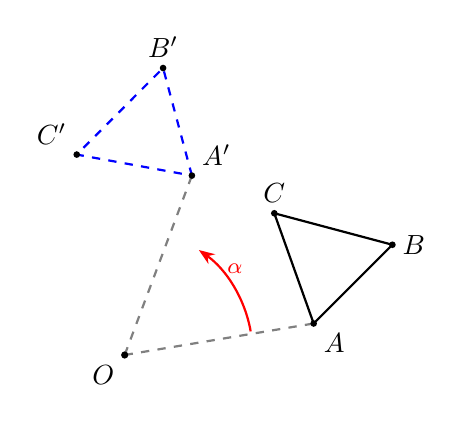
\begin{tikzpicture}[scale=1.0, thick]
  \coordinate (O) at (0,0);
  \coordinate (A) at (2.4, 0.4);
  \coordinate (B) at (3.4, 1.4);
  \coordinate (C) at (1.9, 1.8);
  % 旋转角 60° 逆时针
  \coordinate (Ap) at ({2.4*cos(60)-0.4*sin(60)}, {2.4*sin(60)+0.4*cos(60)});
  \coordinate (Bp) at ({3.4*cos(60)-1.4*sin(60)}, {3.4*sin(60)+1.4*cos(60)});
  \coordinate (Cp) at ({1.9*cos(60)-1.8*sin(60)}, {1.9*sin(60)+1.8*cos(60)});

  \draw (A) -- (B) -- (C) -- cycle;
  \draw[blue, dashed] (Ap) -- (Bp) -- (Cp) -- cycle;

  \draw[gray, dashed] (O) -- (A);
  \draw[gray, dashed] (O) -- (Ap);
  \draw[red, -{Stealth[length=2mm]}] (1.6,0.3) arc (10:55:1.6);
  \node[red] at (1.4,1.1) {\footnotesize $\alpha$};

  \fill (O) circle (1.3pt);
  \fill (A) circle (1.2pt); \fill (B) circle (1.2pt); \fill (C) circle (1.2pt);
  \fill (Ap) circle (1.2pt); \fill (Bp) circle (1.2pt); \fill (Cp) circle (1.2pt);
  \node[below left]  at (O) {$O$};
  \node[below right] at (A) {$A$};
  \node[right]       at (B) {$B$};
  \node[above]       at (C) {$C$};
  \node[above right] at (Ap) {$A'$};
  \node[above]       at (Bp) {$B'$};
  \node[above left]  at (Cp) {$C'$};
\end{tikzpicture}
\end{document}
